\documentclass[11pt]{article}
\usepackage{amsmath,amssymb}
\usepackage{tikz}
\makeatletter
\newcommand\report[2]{%
  \pgfextractx{\dimen0}{\pgfpointanchor{#1}{center}}%
  \pgfextracty{\dimen2}{\pgfpointanchor{#1}{center}}%
  \pgfextractx{\dimen4}{\pgfpointdiff{\pgfpointanchor{#1}{center}}{\pgfpointanchor{#1}{east}}}%
  \pgfextracty{\dimen6}{\pgfpointdiff{\pgfpointanchor{#1}{center}}{\pgfpointanchor{#1}{north}}}%
  \typeout{GOT #2 X=\the\dimen0 Y=\the\dimen2 E=\the\dimen4 N=\the\dimen6}}
\makeatother
\usetikzlibrary{positioning}
\begin{document}
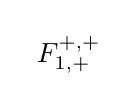
\begin{tikzpicture}
  \coordinate (t) at (0,0);
  \node[] (n) at (3cm, 1cm) {$F_{1,+}^{+,+}$};
  \report{n}{0}
\end{tikzpicture}
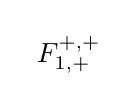
\begin{tikzpicture}
  \coordinate (t) at (0,0);
  \node[anchor=west] (n) at (3cm, 1cm) {$F_{1,+}^{+,+}$};
  \report{n}{1}
\end{tikzpicture}
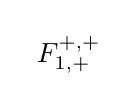
\begin{tikzpicture}
  \coordinate (t) at (0,0);
  \node[anchor=north] (n) at (3cm, 1cm) {$F_{1,+}^{+,+}$};
  \report{n}{2}
\end{tikzpicture}
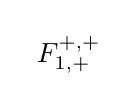
\begin{tikzpicture}
  \coordinate (t) at (0,0);
  \node[anchor=north east] (n) at (3cm, 1cm) {$F_{1,+}^{+,+}$};
  \report{n}{3}
\end{tikzpicture}
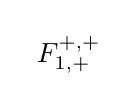
\begin{tikzpicture}
  \coordinate (t) at (0,0);
  \node[above] (n) at (3cm, 1cm) {$F_{1,+}^{+,+}$};
  \report{n}{4}
\end{tikzpicture}
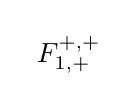
\begin{tikzpicture}
  \coordinate (t) at (0,0);
  \node[above=20pt] (n) at (3cm, 1cm) {$F_{1,+}^{+,+}$};
  \report{n}{5}
\end{tikzpicture}
\end{document}
